%% LyX 2.1.3 created this file.  For more info, see http://www.lyx.org/.
%% Do not edit unless you really know what you are doing.
\documentclass[11pt,english]{article}
\renewcommand{\rmdefault}{cmr}
\renewcommand{\sfdefault}{cmss}
\renewcommand{\ttdefault}{cmtt}
\usepackage[T1]{fontenc}
\usepackage[latin9]{inputenc}
\usepackage{geometry}
\geometry{verbose,tmargin=2.5cm,bmargin=2.5cm,lmargin=2.5cm,rmargin=2.5cm}
\setlength{\parskip}{\bigskipamount}
\setlength{\parindent}{0pt}
\usepackage{babel}
\usepackage{amsthm}
\usepackage{amsmath}
\usepackage{amssymb}
\usepackage{setspace}
\setstretch{0.96}
\usepackage[unicode=true,pdfusetitle,
 bookmarks=true,bookmarksnumbered=false,bookmarksopen=false,
 breaklinks=false,pdfborder={0 0 0},backref=false,colorlinks=false]
 {hyperref}

\makeatletter
%%%%%%%%%%%%%%%%%%%%%%%%%%%%%% Textclass specific LaTeX commands.
\theoremstyle{plain}
\newtheorem{thm}{\protect\theoremname}
  \theoremstyle{plain}
  \newtheorem{cor}[thm]{\protect\corollaryname}
  \theoremstyle{plain}
  \newtheorem{lem}[thm]{\protect\lemmaname}
  \theoremstyle{plain}
  \newtheorem{prop}[thm]{\protect\propositionname}
  \theoremstyle{plain}
  \newtheorem{conjecture}[thm]{\protect\conjecturename}
  \theoremstyle{definition}
  \newtheorem{defn}[thm]{\protect\definitionname}
  \theoremstyle{definition}
  \newtheorem{example}[thm]{\protect\examplename}
  \theoremstyle{remark}
  \newtheorem{rem}[thm]{\protect\remarkname}
  \theoremstyle{remark}
  \newtheorem{claim}[thm]{\protect\claimname}

%%%%%%%%%%%%%%%%%%%%%%%%%%%%%% User specified LaTeX commands.
\date{}

% cleveref allows \ref{thm:asdf} instead of Theorem~\ref{thm:asdf}
\usepackage[nameinlink,capitalise,noabbrev]{cleveref}
\AtBeginDocument{\renewcommand{\ref}[1]{\cref{#1}}}

\usepackage[parfill]{parskip}
\setlength{\parskip}{\bigskipamount}

%have space before theorems
\begingroup
    \makeatletter
    \@for\theoremstyle:=definition,remark,plain\do{%
        \expandafter\g@addto@macro\csname th@\theoremstyle\endcsname{%
            \addtolength\thm@preskip\parskip
            }%
        }
\endgroup

% LyX won't let me include cleveref before theorem declarations so I need to redefine everything as a hack
\theoremstyle{plain}
\newtheorem{mythm}{\protect\theoremname}
\renewenvironment{thm}{\begin{mythm}}{\end{mythm}}
\crefname{mythm}{Theorem}{Theorems}
\theoremstyle{definition}
\newtheorem{mydefn}[mythm]{\protect\definitionname}
\renewenvironment{defn}{\begin{mydefn}}{\end{mydefn}}
\theoremstyle{definition}
\newtheorem{myexample}[mythm]{\protect\examplename}
\renewenvironment{example}{\begin{myexample}}{\end{myexample}}
\theoremstyle{plain}
\newtheorem{myprop}[mythm]{\protect\propositionname}
\renewenvironment{prop}{\begin{myprop}}{\end{myprop}}
\theoremstyle{plain}
\newtheorem{mycor}[mythm]{\protect\corollaryname}
\renewenvironment{cor}{\begin{mycor}}{\end{mycor}}
\theoremstyle{plain}
\newtheorem{mylem}[mythm]{\protect\lemmaname}
\renewenvironment{lem}{\begin{mylem}}{\end{mylem}}
\crefname{mylem}{Lemma}{Lemmas}
\theoremstyle{plain}
\newtheorem{myconjecture}[mythm]{\protect\conjecturename}
\renewenvironment{conjecture}{\begin{myconjecture}}{\end{myconjecture}}
\theoremstyle{remark}
\newtheorem{myrem}[mythm]{\protect\remarkname}
\renewenvironment{rem}{\begin{myrem}}{\end{myrem}}
\theoremstyle{plain}
\newtheorem{myclaim}[mythm]{\protect\claimname}
\renewenvironment{claim}{\begin{myclaim}}{\end{myclaim}}

% equation cref format
\crefformat{equation}{#2(#1)#3}

% \left(\right) should behave the same as ()
\let\originalleft\left
\let\originalright\right
\renewcommand{\left}{\mathopen{}\mathclose\bgroup\originalleft}
\renewcommand{\right}{\aftergroup\egroup\originalright}
\usepackage{pgfplots}
\usetikzlibrary{pgfplots.groupplots}
\usepackage{verbatim}

%make sure tildes in url are vertically centered
\makeatletter
\renewcommand*{\UrlTildeSpecial}{%
  \do\~{%
    \mbox{%
      \fontfamily{ptm}\selectfont
      \textasciitilde
    }%
  }%  
}%    
\let\Url@force@Tilde\UrlTildeSpecial
\makeatother

%graph drawing
\usepackage{tikz}
%\usetikzlibrary{external}
\usetikzlibrary{decorations.markings}
%\usetikzlibrary{arrows.meta}
%\tikzexternalize
\tikzstyle{vertex}=[circle,draw=black,fill=black,inner sep=0,minimum size=0.2cm,text=white,font=\footnotesize]

%caption labels
\usepackage[labelfont=bf,labelsep=period]{caption}

\usepackage[nomessages]{fp}

\usepackage{calc}

\makeatother

  \providecommand{\claimname}{Claim}
  \providecommand{\conjecturename}{Conjecture}
  \providecommand{\corollaryname}{Corollary}
  \providecommand{\definitionname}{Definition}
  \providecommand{\examplename}{Example}
  \providecommand{\lemmaname}{Lemma}
  \providecommand{\propositionname}{Proposition}
  \providecommand{\remarkname}{Remark}
\providecommand{\theoremname}{Theorem}

\begin{document}

\title{Bounded-degree spanning trees in randomly perturbed graphs}


\author{Michael Krivelevich, Matthew Kwan, Benny Sudakov}

\maketitle
\global\long\def\RR{\mathbb{R}}


\global\long\def\QQ{\mathbb{Q}}


\global\long\def\HH{\mathbb{H}}


\global\long\def\E{\mathbb{E}}


\global\long\def\Var{\operatorname{Var}}


\global\long\def\CC{\mathbb{C}}


\global\long\def\NN{\mathbb{N}}


\global\long\def\ZZ{\mathbb{Z}}


\global\long\def\GG{\mathbb{G}}


\global\long\def\BB{\mathbb{B}}


\global\long\def\DD{\mathbb{D}}


\global\long\def\cL{\mathcal{L}}


\global\long\def\supp{\operatorname{supp}}


\global\long\def\one{\boldsymbol{1}}


\global\long\def\range#1{\left[#1\right]}


\global\long\def\d{\operatorname{d}}


\global\long\def\falling#1#2{\left(#1\right)_{#2}}


\global\long\def\f{\mathbf{f}}


\global\long\def\im{\operatorname{im}}


\global\long\def\sp{\operatorname{span}}


\global\long\def\sign{\operatorname{sign}}


\global\long\def\mod{\operatorname{mod}}


\global\long\def\id{\operatorname{id}}


\global\long\def\disc{\operatorname{disc}}


\global\long\def\lindisc{\operatorname{lindisc}}


\global\long\def\tr{\operatorname{tr}}


\global\long\def\adj{\operatorname{adj}}


\global\long\def\Unif{\operatorname{Unif}}


\global\long\def\Po{\operatorname{Po}}


\global\long\def\Bin{\operatorname{Bin}}


\global\long\def\Ber{\operatorname{Ber}}


\global\long\def\Geom{\operatorname{Geom}}


\global\long\def\Hom{\operatorname{Hom}}


\global\long\def\floor#1{\left\lfloor #1\right\rfloor }


\global\long\def\ceil#1{\left\lceil #1\right\rceil }


\global\long\def\flip#1{\overline{#1}}


\global\long\def\a{\alpha}


\global\long\def\c{c}


\global\long\def\D{\Delta}


\global\long\def\G{G}


\global\long\def\F{F}


\global\long\def\T{T}


\global\long\def\R{R}


\global\long\def\B#1{\Gamma_{A,B}\left(#1\right)}

\begin{abstract}
We show that for any bounded-degree spanning tree $T$ and any fixed
dense graph $G$, a modest random perturbation of $G$ will typically
contain a copy of $T$. This combines the viewpoints of the well-studied
problems of embedding trees into fixed dense graphs and into random
graphs, and extends a sizeable body of existing research on randomly
perturbed graphs. Specifically, we show that there is $\c=\c\left(\a,\D\right)$
such that if $\G$ is an $n$-vertex graph with minimum degree at
least $\a n$, and $\T$ is an $n$-vertex tree with maximum degree
at most $\D$, then if we add $\c n$ uniformly random edges to $\G$,
the resulting graph will contain $\T$ asymptotically almost surely
(as $n\to\infty$). Our proof uses a lemma concerning the decomposition
of a dense graph into super-regular pairs of comparable sizes, which
may be of independent interest.
\end{abstract}
\begin{comment}
\begin{thm}
t\end{thm}
\begin{cor}
c\end{cor}
\begin{lem}
l\end{lem}
\begin{prop}
p\end{prop}
\begin{conjecture}
c\end{conjecture}
\begin{defn}
d\end{defn}
\begin{example}
e\end{example}
\begin{rem}
r\end{rem}
\begin{claim}
c
\end{claim}
\end{comment}


\section{Introduction}

A classical theorem of Dirac \cite{Dir52} states that any $n$-vertex
graph ($n\ge3$) with minimum degree at least $n/2$ has a Hamilton
cycle: a cycle that passes through all the vertices of the graph.
More recently, there have been many results showing that this kind
of minimum degree condition is sufficient to guarantee the existence
of different kinds of spanning graphs. For example, in \cite[Theorem~1$'$]{KSS95}
Koml\'os, S\'ark\"ozy and Szemer\'edi proved that for any $\Delta$
and $\gamma>0$, any $n$-vertex graph ($n$ sufficiently large) with
minimum degree $\left(1/2+\gamma\right)n$ contains every spanning
tree which has maximum degree at most $\Delta$. This has also been
generalized further in two directions. In \cite{KSS01} Koml\'os,
S\'ark\"ozy and Szemer\'edi improved their result to to allow $\Delta$
to grow with $n$, and in \cite{BST09} B\"ottcher, Schacht and Taraz
gave a result for much more general spanning subgraphs than trees
(see also a result \cite{Csa08} due to Csaba).

The constant $1/2$ in the above Dirac-type theorems is tight: in
order to guarantee the existence of these spanning subgraphs we require
very strong density conditions. But the situation is very different
for a ``typical'' large graph. If we fix an arbitrarily small $\alpha>0$
and select a graph uniformly at random among the (labelled) graphs
with $n$ vertices and $\alpha{n \choose 2}$ edges, then the degrees
will probably each be about $\alpha n$. Such a random graph is Hamiltonian
with probability $1-o\left(1\right)$ (we say it is Hamiltonian \emph{asymptotically
almost surely}, or \emph{a.a.s.}). This follows from a stronger result
by P\'osa \cite{Pos76} that gives a \emph{threshold} for Hamiltonicity:
a random $n$-vertex, $m$-edge graph is Hamiltonian a.a.s. if $m\gg n\log n$,
and fails to be Hamiltonian a.a.s. if $m\ll n\log n$. Although the
exact threshold for bounded-degree spanning trees is not known, in
\cite{Mon14} Montgomery proved that for any $\Delta$ and any tree
$T$ with maximum degree at most $\Delta$, a random $n$-vertex graph
with $\Delta n\left(\log n\right)^{5}$ edges a.a.s. contains $T$.
Here and from now on, all asymptotics are as $n\to\infty$, and we
implicitly round large quantities to integers.

In \cite{BFM03}, Bohman, Frieze and Martin studied Hamiltonicity
in the random graph model that starts with a dense graph and adds
$m$ random edges. This model is a natural generalization of the ordinary
random graph model where we start with nothing, and offers a ``hybrid''
perspective combining the extremal and probabilistic settings of the
last two paragraphs. The model has since been studied in a number
of other contexts; see for example \cite{BHM04,KST06,KKS15}. A property
that holds a.a.s. with small $m$ in our random graph model can be
said to hold not just for a ``globally'' typical graph but for the
typical graph in a small ``neighbourhood'' of our space of graphs.
This tells us that the graphs which fail to satisfy our property are
in some sense ``fragile''. We highlight that it is generally very
easy to transfer results from our model of random perturbation to
other natural models, including those that delete as well as add edges
(this can be accomplished with standard coupling and conditioning
arguments). We also note that a particularly important motivation
is the notion of \emph{smoothed analysis} of algorithms introduced
by Spielman and Teng in \cite{ST04}. This is is a hybrid of worst-case
and average-case analysis, studying the performance of algorithms
in the more realistic setting of inputs that are ``noisy'' but not
completely random.

The statement of \cite[Theorem~1]{BFM03} is that for every $\alpha>0$
there is $c=c\left(\alpha\right)$ such that if we start with a graph
with minimum degree at least $\alpha n$ and add $cn$ random edges,
then the resulting graph will a.a.s. be Hamiltonian. This saves a
logarithmic factor over the usual model where we start with the empty
graph. Note that some dense graphs require a linear number of extra
edges to become Hamiltonian (consider for example the complete bipartite
graph with partition sizes $n/3$ and $2n/3$), so the order of magnitude
of this result is tight.

Let $\GG\left(n,p\right)$ be the binomial random graph model with
vertex set $\range n=\left\{ 1,\dots,n\right\} $, where each edge
is present independently and with probability $p$. (For our purposes
this is equivalent to the model that uniformly at random selects a
$p{n \choose 2}$-edge graph on the vertex set $\range n$). In this
paper we prove the following theorem, extending the aforementioned
result to bounded-degree spanning trees.
\begin{thm}
\label{thm:main-theorem}There is $\c=\c\left(\a,\D\right)$ such
that if $\G$ is a graph on the vertex set $\range n$ with minimum
degree at least $\a n$, and $\T$ is an $n$-vertex tree with maximum
degree at most $\D$, and $\R\in\GG\left(n,\c/n\right)$, then a.a.s.
$\T\subseteq\G\cup\R$.
\end{thm}
One of the ingredients of the proof is the following lemma, due to
Alon and two of the authors (\cite[Theorem~1.1]{AKS07}). It shows
that the random edges in $\R$ are already enough to embed almost-spanning
trees.
\begin{lem}
\label{lem:almost-spanning}There is $\c=\c\left(\varepsilon,\D\right)$
such that $\G\in\GG\left(n,\c/n\right)$ a.a.s. contains every tree
of maximum degree at most $\D$ on $\left(1-\varepsilon\right)n$
vertices.
\end{lem}
We will split the proof of \ref{thm:main-theorem} into two cases
in a similar way to \cite{Kri10}. If our spanning tree $\T$ has
many leaves, then we remove the leaves and embed the resulting non-spanning
tree in $\R$ using \ref{lem:almost-spanning}. To complete this into
our spanning tree $\T$, it remains to match the the vertices needing
leaves with leftover vertices. This amounts to finding a perfect matching
in a certain bipartite graph. The random edges in $\R$ provide several
almost-perfect matchings on their own; we combine these with the dense
graph $\G$ to satisfy the conditions of Hall's marriage theorem and
guarantee the required perfect matching. The details for this case
are given in \ref{sub:many-leaves}.

The more difficult case is where $\T$ has few leaves, which we attack
in \ref{sub:few leaves}. In this case $\T$ cannot be very ``complicated''
and must be a subdivision of a small tree. In particular $\T$ must
have many long \emph{bare paths}: paths where each vertex has degree
exactly two. By removing these bare paths we obtain a small forest
which we can embed into $\R$ using \ref{lem:almost-spanning} (the
details are in \ref{sub:embed-forest}). In order to complete this
forest into our spanning tree $\T$, we need to join up distinguished
``special pairs'' of vertices with disjoint paths of certain lengths.

In order to make this task feasible, in \ref{sub:partition-into-blobs}
we first use Szemer\'edi's regularity lemma to divide the vertex
set into a bounded number of ``clusters'', which we can partition
into ``super-regular pairs'' (basically, dense subgraphs with edges
very well-distributed in $\G$). After embedding our small forest,
In \ref{sub:fix-endpoints} we find some short paths that effectively
``move'' the special pairs we need to join up. We do this in such
a way that it remains to join up special pairs of vertices which are
each fully contained in one of the super-regular cluster-pairs with
which we partitioned $\G$. Combining the super-regularity in the
cluster-pairs with the random edges in $\R$, in \ref{sub:cluster-adjustment}
we can then greedily find many of our desired paths. We carefully
set aside some of these special paths in such a way that the numbers
of vertices remaining in each cluster satisfy certain divisibility
requirements. From here the super-regularity of the pairs allows us
to find the rest of our paths using a tool called the ``blow-up lemma''
(\ref{sub:blow-up}).


\section{Proof of \texorpdfstring{}{Theorem~}\ref{thm:main-theorem}}

We split the random edges into multiple independent ``phases'':
say $\R\supseteq\R_{1}\cup\R_{2}\cup\R_{3}\cup\R_{4}$, where $\R_{i}\in\GG\left(n,\c_{i}/n\right)$
for some large $\c_{i}=\c_{i}\left(\a,\D\right)$ to be determined
later (these $\c_{i}$ will in turn determine $\c$). Let $V=\range n$
be the common vertex set of $\G$, $\R$ and the $\R_{i}$.
\begin{rem}
\label{rem:symmetry}At several points in the proof we will prove
that (with high probability) there exist certain substructures in
the random edges $\R$, and we will assume by symmetry that these
substructures (or some corresponding vertex sets) are themselves uniformly
random. A simple way to see why this kind of reasoning is valid is
to notice that if we apply a uniformly random vertex permutation to
a random graph $\R\in\GG\left(n,p\right)$, then by symmetry the resulting
distribution is still $\GG\left(n,p\right)$. So we can imagine that
we are finding substructures in an auxiliary random graph, then randomly
mapping these structures to our vertex set.
\end{rem}

\subsection{Case 1: $\protect\T$ has many leaves\label{sub:many-leaves}}

For our first case suppose there are at least $\lambda n$ leaves
in $\T$ (for some fixed $\lambda=\lambda\left(\a\right)>0$ which
will be determined in the second case). Then consider a tree $\T'$
with some $\lambda n$ leaves removed. By \ref{lem:almost-spanning}
we can a.a.s. embed $\T'$ into $\R_{1}$ (we also denote this embedded
subgraph by $\T'$). Let $A\subseteq V$ be the set of vertices of
$\T'$ which had a leaf deleted from them, and for $a\in A$ let $\ell\left(a\right)\le\Delta$
be the number of leaves that were deleted from $a$. Let $B\subseteq V$
be the set of $\lambda n$ vertices not part of $\T'$. In order to
complete the embedding of $\T'$ into an embedding of $\T$ it suffices
to find a set of disjoint stars in $\G\cup\R_{2}$ each with a center
vertex $a\in A$ and with $\ell\left(a\right)$ leaves in $B$. We
will prove the existence of such stars with the following Hall-type
condition.
\begin{lem}
\label{lem:hall-stars}Consider a bipartite graph $\G$ with bipartition
$A\cup B$, and consider a function $\ell:A\to\NN$ such that $\sum_{a\in A}\ell\left(a\right)=\left|B\right|$.
Suppose that 
\[
\left|N\left(S\right)\right|\ge\sum_{s\in S}\ell\left(s\right)\quad\mbox{for all }S\subseteq A.
\]
Then there is a set of disjoint stars in $\G$, each of which has
a center vertex $a\in A$ and $\ell\left(a\right)$ leaves in $B$.
\end{lem}
\ref{lem:hall-stars} can be easily proved by applying Hall's marriage
theorem to an auxiliary bipartite graph which has $\ell\left(a\right)$
copies of each vertex $a\in A$.

We can assume $A$ and $B$ are uniformly random disjoint subsets
of $V$ of their size (note $\left|A\right|\ge\lambda n/\D$ and $\left|B\right|=\lambda n$).
For each $a\in A$, the random variable $\left|N_{\G}\left(a\right)\cap B\right|$
is hypergeometrically distributed with expected value at least $\lambda\a n$,
and similarly each $\left|N_{\G}\left(b\right)\cap A\right|$ ($b\in B$)
is hypergeometric with expectation at least $\lambda\a n/\D$. Let
$\beta=\lambda\a/\left(2\D\right)$; by a concentration inequality
(for example, see \cite[Theorem 2.10]{JLR00}) and the union bound,
in $\G$ each $a\in A$ a.a.s. has at least $\beta n$ neighbours
in $B$, and each $b\in B$ a.a.s. has at least $\beta n$ neighbours
in $A$. That is to say, the bipartite graph induced by $\G$ on the
bipartition $A\cup B$ has minimum degree at least $\beta n$. We
treat $A$ and $B$ as fixed sets satisfying this property. It suffices
to prove the following lemma.
\begin{lem}
\label{lem:bipartite-perturbed-stars}For any $\beta>0$ and $\Delta\in\RR$
there is $\c=\c\left(\beta\right)$ such that the following holds.
Suppose $\G$ is a bipartite graph with bipartition $A\cup B$ ($\left|A\right|,\left|B\right|\le n$)
and minimum degree at least $\beta n$. Suppose $\ell:A\to\range{\Delta}$
is some function satisfying $\sum_{a\in A}\ell\left(a\right)=\left|B\right|$.
Let $\R$ be the random bipartite graph where each edge between $A$
and $B$ is present independently and with probability $\c/n$. Then
a.a.s. $\G\cup\R$ satisfies the condition in \ref{lem:hall-stars}.\end{lem}
\begin{proof}
Let $S\subseteq A$ be nonempty. If $\left|S\right|\le\beta n/\Delta$
then $\left|N_{\G}\left(S\right)\right|\ge\left|N_{\G}\left(a\right)\right|\ge\beta n\ge\sum_{s\in S}\ell\left(s\right)$
for any $a\in S$. If $\left|S\right|\ge\left|A\right|-\beta n$ then
$\left|A\backslash S\right|\le\left|N_{\G}\left(b\right)\right|$
for each $b\in B$, so $\left|N_{\G}\left(S\right)\right|=\left|B\right|\ge\sum_{s\in S}\ell\left(s\right)$.

The remaining case is where $\beta n/\Delta\le\left|S\right|\le\left|A\right|-\beta n$.
In this case $\sum_{s\in S}\ell\left(s\right)=\left|B\right|-\sum_{a\in A\backslash S}\ell\left(a\right)\le\left|B\right|-\beta n$.
Now, for any subsets $A'\subseteq A$ and $B'\subseteq B$ with $\left|A'\right|=\beta n/\Delta$
and $\left|B'\right|=\beta n$, the probability there is no edge between
$A'$ and $B'$ is $\left(1-\c/n\right)^{\left(\beta n/\Delta\right)\left(\beta n\right)}\le e^{-\c\beta^{2}n/\Delta}$.
There are at most $2^{2n}$ choices of such $A',B'$, so for large
$\c$, by the union bound there is a.a.s. an edge between any such
pair of sets. If this is true, it follows that $\left|N_{\R}\left(S\right)\right|\ge\left|B\right|-\beta n$,
because if $S$ had more than $\beta n$ non-neighbours in $B$ then
this would give us a contradictory pair of subsets with no edge between
them. We have proved that a.a.s. $\left|N_{\R}\left(S\right)\right|\ge\sum_{s\in S}\ell\left(s\right)$
for all $S\subseteq A$, as required.
\end{proof}

\subsection{Case 2: $\protect\T$ has few leaves\label{sub:few leaves}}

Now we address the second case where there are fewer than $\lambda n$
leaves in $\T$.


\subsubsection{Partitioning into super-regular pairs\label{sub:partition-into-blobs}}

As outlined in the introduction, we first need to divide $\G$ into
a bounded number of pairs of ``partner clusters'' with edges well-distributed
between them.

\global\long\def\h{h}

\begin{defn}
For a disjoint pair of vertex sets $\left(X,Y\right)$ in a graph
$G$, let its \emph{density} $d\left(X,Y\right)$ be the number of
edges between $X$ and $Y$, divided by $\left|X\right|\left|Y\right|$.
A pair of vertex sets $\left(V_{1},V_{2}\right)$ is said to be \emph{$\varepsilon$-regular}
in $G$ if for any $U_{1},U_{2}$ with $U_{\h}\subseteq V_{\h}$ and
$\left|U_{\h}\right|\ge\varepsilon\left|V_{\h}\right|$, we have $\left|d\left(U_{1},U_{2}\right)-d\left(V_{1},V_{2}\right)\right|\le\varepsilon$.
If alternatively $d\left(U_{1},U_{2}\right)\ge\delta$ for all such
pairs $U_{1},U_{2}$ then we say $\left(V_{1},V_{2}\right)$ is \emph{$\left(\varepsilon,\delta\right)$-dense}.
Let $\flip{\h}=2-\h$; if $\left(V_{1},V_{2}\right)$ is $\left(\varepsilon,\delta\right)$-dense
and moreover each $v\in V_{\h}$ has at least $\delta\left|V_{\flip{\h}}\right|$
neighbours in $V_{\flip{\h}}$, then we say $\left(V_{1},V_{2}\right)$
is \emph{$\left(\varepsilon,\delta\right)$-super-regular}.\end{defn}
\begin{lem}
\label{lem:partition-into-blobs}For $\a,\varepsilon>0$ with $\varepsilon$
sufficiently small relative to $\a$, there are $\delta=\delta\left(\a\right)>0$,
$\rho=\rho\left(\a\right)$ and $Q=Q\left(\a,\varepsilon\right)$,
such that the following holds. Let $\G$ be an $n$-vertex graph with
minimum degree at least $\a n$. Then there is $q\le Q$ and a partition
of $V\left(\G\right)$ into clusters $V_{i}^{\h}$ ($1\le i\le q$,
$\h=1,2$) such that each $\left|V_{i}^{\h}\right|=\Theta\left(n\right)$
and each pair $\left(V_{i}^{1},V_{i}^{2}\right)$ is $\left(\varepsilon,\delta\right)$-super-regular.
Moreover, each $\left|V_{i}^{\h}\right|/\left|V_{j}^{g}\right|\le\rho$.
\end{lem}
We emphasize that in \ref{lem:partition-into-blobs} we do \emph{not
}guarantee that the sets $V_{i}^{\h}$ are of the same size, just
that the variation in the sizes of the clusters is bounded independently
of $\varepsilon$.

To prove \ref{lem:partition-into-blobs}, we will apply Szemer\'edi's
regularity lemma to obtain a reduced \emph{cluster graph}, then decompose
this cluster graph into small stars. In each star $T_{i}$, the center
cluster will correspond to $V_{i}^{1}$ and the leaf clusters will
be combined to form $V_{i}^{2}$. We will then have to redistribute
some of the vertices to ensure super-regularity. Before giving the
details of the proof, we give a statement of (a version of) Szemer\'edi's
regularity lemma and some auxiliary lemmas for working with regularity
and super-regularity.
\begin{lem}[Szemer\'edi's regularity lemma, minimum degree form]
\label{lem:szemeredi-regularity}For every $\a>0$, and any $\varepsilon>0$
that is sufficiently small relative to $\a$, there are $\a'=\a'\left(\a\right)>0$
and $K=K\left(\varepsilon\right)$ such that the following holds.
For any graph $\G$ of minimum degree at least $\a\left|\G\right|$,
there is a partition of $V\left(\G\right)$ into clusters $V_{0},V_{1},\dots V_{k}$
($k\le K$), and a spanning subgraph $\G'$ of $\G$, satisfying the
following properties. The ``exceptional cluster'' $V_{0}$ has size
at most $\varepsilon n$, and the other clusters have equal size $sn$.
The minimum degree of $\G'$ is at least $\a'n$. There are no edges
of $\G'$ within the clusters, and each pair of non-exceptional clusters
is $\varepsilon$-regular in $\G'$ with density zero or at least
$\a'$. Moreover, define the \emph{cluster graph} $C$ as the graph
whose vertices are the $k$ non-exceptional clusters $V_{i}$, and
whose edges are the pairs of clusters between which there is nonzero
density in $\G'$. The minimum degree of $C$ is at least $\a'k$.
\end{lem}
This version of Szemer\'edi's regularity lemma is just the ``degree
form'' of \cite[Theorem~1.10]{KS96}, plus a straightforward claim
about minimum degree. Our statement follows directly from \cite[Proposition~9]{KOT05}.

Before we proceed to the proof of \ref{lem:partition-into-blobs},
we give some simple lemmas about $\left(\varepsilon,\delta\right)$-denseness.
Note that $\left(\varepsilon,\delta\right)$-denseness is basically
a one-sided version of $\varepsilon$-regularity that is more convenient
in proofs about super-regularity. In particular, an $\varepsilon$-regular
pair with density $\delta$ is $\left(\varepsilon,\delta-\varepsilon\right)$-dense.
Here and in later sections, most of the theorems about $\left(\varepsilon,\delta\right)$-dense
pairs correspond to analogous theorems for $\varepsilon$-regular
pairs with density about $\delta$.
\begin{lem}
\label{lem:combine-clusters}Suppose $V_{1}^{2},\dots,V_{r}^{2}$
are disjoint clusters of the same sizes such that each $\left(V^{1},V_{i}^{2}\right)$
is $\left(\varepsilon,\delta\right)$-dense. Let $V^{2}=\bigcup_{i=1}^{r}V_{i}^{2}$;
then $\left(V^{1},V^{2}\right)$ is $\left(\varepsilon,\delta/r\right)$-dense.\end{lem}
\begin{proof}
Let $U^{\h}\subseteq V^{\h}$ with $\left|U^{\h}\right|\ge\varepsilon\left|V^{\h}\right|$.
Let $V_{i}^{2}$ be the cluster which has the largest intersection
with $U^{2}$, so we have $\left|U^{2}\cap V_{i}^{2}\right|\ge\varepsilon\left|V^{2}\right|/r=\varepsilon\left|V_{i}^{2}\right|$,
and there are therefore at least $\delta\left|U^{1}\right|\left|U^{2}\cap V_{i}^{2}\right|\ge\left(\delta/r\right)\left|U^{1}\right|\left|U^{2}\right|$
edges between $U^{1}$ and $U^{2}$.\end{proof}
\begin{lem}
\label{lem:robust-regular}Let $\left(V^{1},V^{2}\right)$ be an $\left(\varepsilon,\delta\right)$-super-regular
pair. Suppose we have $W^{\h}\supseteq V^{\h}$ with $\left|W^{\h}\right|\le\left(1+f\varepsilon\right)\left|V^{\h}\right|$,
and suppose that each vertex in $W^{\h}\backslash V^{\h}$ has at
least $\delta'\left|W^{\flip{\h}}\right|$ neighbours in $W^{\flip{\h}}$.
Then $\left(W^{1},W^{2}\right)$ is an $\left(\varepsilon',\delta'\right)$-super-regular
pair, where 
\[
\varepsilon'=\max\left\{ 2f,1+f\right\} \,\varepsilon,\quad\delta'=\min\left\{ 1/4,1/\left(1+f\varepsilon\right)\right\} \,\delta.
\]
\end{lem}
\begin{proof}
Suppose $U^{\h}\subseteq W^{\h}$ with $\left|U^{\h}\right|\ge\varepsilon'\left|W^{\h}\right|$.
Then $\left|U^{\h}\cap V^{\h}\right|\ge\varepsilon'\left|W^{\h}\right|-f\varepsilon\left|V^{\h}\right|\ge\varepsilon\left|V^{\h}\right|$
so there are at least $\delta\left|U^{1}\cap V^{1}\right|\left|U^{2}\cap V^{2}\right|$
edges between $U^{1}$ and $U^{2}$. But note that $\left|U^{\h}\cap V^{\h}\right|\ge\left|U^{\h}\right|-f\varepsilon\left|W^{\h}\right|\ge\left(1-\left(f\varepsilon\right)/\varepsilon'\right)\left|U^{\h}\right|\ge\left(1/2\right)\left|U^{\h}\right|$,
so $d\left(U^{1},U^{2}\right)\ge\delta/4$ and $\left(W^{1},W^{2}\right)$
is $\left(\varepsilon',\delta'\right)$-dense.

Next, note that each $v\in V^{\h}$ has $\delta\left|V^{\flip{\h}}\right|\ge\delta'\left|W^{\flip{\h}}\right|$
neighbours in $W^{\flip{\h}}$, and by assumption each $v\in W^{\h}\backslash V^{\h}$
has $\delta'\left|W^{\flip{\h}}\right|$ neighbours in $W^{\flip{\h}}$,
proving that $\left(W^{1},W^{2}\right)$ is $\left(\varepsilon',\delta'\right)$-super-regular.\end{proof}
\begin{lem}
\label{lem:regular-contains-superregular}Every $\left(\varepsilon,\delta\right)$-dense
pair $\left(V^{1},V^{2}\right)$ contains a $\left(\varepsilon/\left(1-\varepsilon\right),\delta-\varepsilon\right)$-super-regular
sub-pair $\left(W^{1},W^{2}\right)$, where $\left|W^{\h}\right|\ge\left(1-\varepsilon\right)\left|V^{\h}\right|$.
\end{lem}
\ref{lem:regular-contains-superregular} follows easily from the same
proof as \cite[Proposition~6]{BST08}.

Now we prove \ref{lem:partition-into-blobs}. First we need a lemma
for our decomposition into small stars.
\begin{lem}
\label{lem:star-cover}Let $G$ be an $n$-vertex graph with minimum
degree at least $\a n$. Then there is a spanning subgraph $S$ which
is a union of vertex-disjoint stars, each with at least two and at
most $1+1/\a$ vertices.\end{lem}
\begin{proof}
Let $S$ be a union of such stars with the maximum number of vertices.
Suppose there is a vertex $v$ uncovered by $S$. If $v$ has a neighbour
which is a center of one of the stars in $S$, and that star has fewer
than $1+\floor{1/\a}$ vertices, then we could add $v$ to that star,
contradicting maximality. (Here we allow either vertex of a 2-vertex
star to be considered the ``center''). Otherwise, if $v$ has a
neighbour $w$ which is a leaf of one of the stars in $S$, then we
could remove that leaf from its star and create a new 2-vertex star
with edge $vw$, again contradicting maximality. The remaining case
is where each of the (at least $\a n$) neighbours of $v$ is a center
of a star with $1+\floor{1/\a}>1/\a$ vertices. But these stars would
comprise more than $n$ vertices, which is again a contradiction.
We conclude that $S$ covers $G$, as desired.
\end{proof}

\begin{proof}[Proof of \ref{lem:partition-into-blobs}]
Apply our minimum degree form of Szemer\'edi's regularity lemma,
with some $\varepsilon'$ to be determined (which we will repeatedly
assume is sufficiently small). Consider a cover of $C$ by stars $T_{1},\dots,T_{q}$
of size at most $1+1/\a'$, as guaranteed by \ref{lem:star-cover}.
Let $W_{i}^{1}$ be the center cluster of $T_{i}$, and let $W_{i}^{2}$
be the union of the leaf clusters of $T_{i}$ (for two-vertex stars,
arbitrarily choose one vertex as the ``leaf'' and one as the ``center'').
Each edge of the cluster graph $C$ corresponds to an $\left(\varepsilon',\a'/2\right)$-dense
pair, and each $W_{i}^{\h}$ is the union of at most $1/\a'$ clusters
$V_{i}$. By \ref{lem:combine-clusters}, with $\delta'=\left(\a'\right)^{2}/2$
each pair $\left(W_{i}^{1},W_{i}^{2}\right)$ is $\left(\varepsilon',\delta'\right)$-dense
in $\G'$ (therefore $\G$).

Apply \ref{lem:regular-contains-superregular} to obtain sets $V_{i}^{\h}\subseteq W_{i}^{\h}$
such that $\left|V_{i}^{\h}\right|=\left(1-\varepsilon'\right)\left|W_{i}^{\h}\right|$
and each $\left(V_{i}^{1},V_{i}^{2}\right)$ is $\left(2\varepsilon',\delta''\right)$-super-regular,
for $\delta''=\delta'/2$. Combining the exceptional cluster $V_{0}$
and all the $W_{i}^{\h}\backslash V_{i}^{\h}$, there are at most
$2\varepsilon'n$ ``bad'' vertices not part of a super-regular pair.

Each bad vertex $v$ has at least $\a'n-2\varepsilon'n$ neighbours
to the clusters $V_{i}^{\h}$. The clusters $V_{i}^{\h}$ which have
fewer than $\delta''\left|V_{i}^{\h}\right|$ such neighbours contain
at most $\delta''n$ of these neighbours. Each $V_{i}^{\h}$ has size
at most $sn/\a'$, so for small $\varepsilon'$ there are at least
\[
\frac{\a'n-2\varepsilon'n-\delta''n}{sn/\a'}\ge\left(\a'\right)^{2}/\left(2s\right)
\]
clusters $V_{i}^{\h}$ which have at least $\delta''\left|V_{i}^{\h}\right|$
neighbours of $v$. Pick one such $V_{i}^{\h}$ uniformly at random,
and put $v$ in $V_{i}^{\flip{\h}}$ (do this independently for each
bad $v$). By a concentration inequality, after this procedure a.a.s.
at most $2\left(2\varepsilon'n\right)/\left(\left(\a'\right)^{2}/\left(2s\right)\right)\le\left(8\varepsilon'/\left(\a'\right)^{2}\right)\left|W_{i}^{\h}\right|\le\left(9\varepsilon'/\left(\a'\right)^{2}\right)\left|V_{i}^{\h}\right|$
bad vertices have been added to each $V_{i}^{\h}$. By \ref{lem:robust-regular},
for small $\varepsilon'$ each $\left(V_{i}^{1},V_{i}^{2}\right)$
is now $\left(O\left(\varepsilon'\right),\delta''/4\right)$-super-regular.
With $\delta=\delta''/4$ and $\varepsilon'$ small relative to $\varepsilon$,
we are done.
\end{proof}
\global\long\def\bi{\mathbf{i}}


\global\long\def\bj{\mathbf{j}}


\global\long\def\br{\mathbf{r}}


We apply \ref{lem:partition-into-blobs} to our graph $\G$, with
$\varepsilon_{1}=\varepsilon_{1}\left(\delta\right)$ to be determined.
For $\bi=\left(i,\h\right)$, let $V_{\bi}=V_{i}^{\h}$, and let $\left|V_{\bi}\right|=s_{\bi}n$.


\subsubsection{Embedding a small subforest of $\protect\T$\label{sub:embed-forest}}

Having fixed our partition of $G$ into $V_{\bi}$, in this section
we will start to embed $\T$ into $\G\cup\R$. Just as in \ref{sub:many-leaves},
we will use the decomposition of $\R$ into ``phases'' $\R_{1},\R_{2},\R_{3},\R_{4}$
(but we start with $\R_{2}$ for consistency with the section numbering).

Recall that a \emph{bare path} in $\T$ is a path $P$ such that every
vertex of $P$ has degree exactly two in $\T$. Proceeding with the
proof outline, we need the fact that $\T$ is almost entirely composed
of bare paths, as is guaranteed by the following lemma due to one
of the authors (\cite[Lemma~2.1]{Kri10}).
\begin{lem}
\label{lem:bare-paths-if-no-leaves}Let $\T$ be a tree on $n$ vertices
with at most $\ell$ leaves. Then $\T$ contains a collection of at
least $\left(n-\left(2\ell-2\right)\left(k+1\right)\right)/\left(k+1\right)$
vertex-disjoint bare paths of length $k$ each.
\end{lem}
\global\long\def\r#1{r\left(#1\right)}


\global\long\def\x{x}


\global\long\def\y{y}


In our case $\ell=\lambda n$. If we choose $k$ large enough and
$\lambda$ small enough, then $\T$ contains a collection of $n/\left(2\left(k-1\right)\right)$
disjoint bare $k$-paths. (The definite value of $k$ will be determined
later; it will depend on $\a$ but not $\varepsilon$). If we delete
the interior vertices of these paths, then we are left with a forest
$\F$ on $n/2$ vertices.

Now, embed $\F$ into the random graph $\R_{2}$. There are $n/\left(2\left(k-1\right)\right)$
``special pairs'' of ``special vertices'' of $\F\subseteq\R_{2}$
that need to be connected with $k$-paths. We call such connecting
paths ``special paths''. Let $X\subseteq V$ be the set of special
vertices and let $W=V\backslash\F$ be the set of ``free'' vertices.
By symmetry we can assume 
\[
X\,\cup\,\F\backslash X\,\cup\,W
\]
is a uniformly random partition of $V$ into parts of sizes $n/\left(k-1\right)$,
$n/2-n/\left(k-1\right)$ and $n/2$ respectively. We can also assume
that the special pairs correspond to a uniformly random partition
of $X$ into pairs. Note that $2\left|W\right|=\left(k-1\right)\left|X\right|$.

Let $X_{\bi}=V_{\bi}\cap X$ and $W_{\bi}=V_{\bi}\backslash F$ be
the set of free vertices remaining in $V_{\bi}$. By a concentration
inequality for the hypergeometric distribution and the union bound,
a.a.s. each $\left|W_{\bi}\right|\sim s_{\bi}n/2$ and $\left|X_{\bi}\right|\sim s_{\bi}n/\left(k-1\right)$.

Here and in future parts of the proof, it is critical that after we
take certain subsets of our super-regular pairs, we maintain super-regularity
or at least density (albeit with weaker $\varepsilon$ and $\delta$).
We will ensure this in each situation by appealing to one of the following
two lemmas.
\begin{lem}
\label{lem:large-preserves-dense}Suppose $\left(V^{1},V^{2}\right)$
is $\left(\varepsilon,\delta\right)$-dense, and let $W^{\h}\subseteq V^{\h}$
with $\left|W^{\h}\right|\ge\gamma\left|V^{\h}\right|$. Then $\left(W^{1},W^{2}\right)$
is $\left(\varepsilon/\gamma,\delta\right)$-dense.\end{lem}
\begin{proof}
If $U^{\h}\subseteq W^{\h}$ with $\left|U^{\h}\right|\ge\left(\varepsilon/\gamma\right)\left|W^{\h}\right|$,
then $\left|U^{\h}\right|\ge\varepsilon\left|V^{\h}\right|$. The
result follows from the definition of $\left(\varepsilon,\delta\right)$-denseness.\end{proof}
\begin{lem}
\label{lem:random-preserves-superregular}Fix $\delta,\varepsilon'>0$.
There is $\varepsilon=\varepsilon\left(\varepsilon'\right)>0$ such
that the following holds. Suppose $\left(V^{1},V^{2}\right)$ is $\left(\varepsilon,\delta\right)$-dense,
let $n_{\h}$ satisfy $\left|V^{\h}\right|\ge n_{\h}=\Omega$$\left(n\right)$
(not necessarily uniformly over $\varepsilon$ and $\delta$) and
for each $\h$ let $W^{\h}\subseteq V^{\h}$ be a uniformly random
subset of size $n_{\h}$. Then $\left(W^{1},W^{2}\right)$ is a.a.s.
$\left(\varepsilon',\delta/2\right)$-dense. If moreover $\left(V^{1},V^{2}\right)$
was $\left(\varepsilon,\delta\right)$-super-regular then $\left(W^{1},W^{2}\right)$
is a.a.s. $\left(\varepsilon',\delta/2\right)$-super-regular.
\end{lem}
\ref{lem:random-preserves-superregular} is a simple consequence of
a highly nontrivial (and much more general) result proved by Gerke,
Kohayakawa, R\"odl and Steger in \cite{GKRS07}, which shows that
small random subsets inherit certain regularity-like properties with
very high probability. The notion of ``lower regularity'' in that
paper essentially corresponds to our notion of $\left(\varepsilon,\delta\right)$-density.
\begin{proof}[Proof of \ref{lem:random-preserves-superregular}]
The fact that $\left(W^{1},W^{2}\right)$ is a.a.s. $\left(\varepsilon',\delta/2\right)$-dense
for suitable $\varepsilon$, follows from two applications of \cite[Theorem~3.6]{GKRS07}.

It remains to consider the degree condition for super-regularity.
For each $v\in W^{\h}$, the number of neighbours of $v$ in $W^{\flip{\h}}$
is hypergeometrically distributed, with expected value at least $\delta n_{\flip{\h}}$.
Since $n_{\flip h}=\Omega\left(n\right)$, a concentration inequality
and the union bound immediately tells us that a.a.s. each such $v$
has $\delta n_{\flip h}/2$ such neighbours, as required.
\end{proof}
Let $\flip{\left(i,\h\right)}=\left(i,\flip{\h}\right)$, and let
$\left[\left(i,\h\right)\right]=i$. It is an immediate consequence
of \ref{lem:random-preserves-superregular} that each $\left(X_{\bi},W_{\flip{\bi}}\right)$
and $\left(W_{\bi},W_{\flip{\bi}}\right)$ are $\left(\varepsilon_{2},\delta_{2}\right)$-super-regular,
where $\delta_{2}=\delta_{1}/2$ and $\varepsilon_{2}$ can be made
arbitrarily small by choice of $\varepsilon_{1}$.

Now that we have embedded $\F$, we no longer care about the vertices
used to embed $\F\backslash X$; they will never be used again. It
is convenient to imagine, for the duration of the proof, that instead
of embedding parts of $\T$, we are ``removing'' vertices from $\G\cup\R$,
gradually making the remaining graph easier to deal with. So, update
$n$ to be the number of vertices not used to embed $\F\backslash X$
(previously $\left(1/2+1/\left(k-1\right)\right)n$), and update $s_{\bi}$
to satisfy $\left|W_{\bi}\right|=s_{\bi}n$. Note that (asymptotically
speaking) this just rescales the $s_{\bi}$ so that they sum to $\left(\left(k-1\right)/\left(k+1\right)\right)n$.
Therefore the variation between the $s_{\bi}$ is still bounded independently
of $\varepsilon$; we can increase $\rho$ slightly so that each $\left|s_{\bi}\right|/\left|s_{\bj}\right|\le\rho$.
We then have $\left|X_{\bi}\right|\sim2s_{\bi}n/\left(k-1\right)$
for each $\bi$, and there are $n/\left(k+1\right)$ special pairs.


\subsubsection{\label{sub:fix-endpoints}Fixing the endpoints of the special paths}

We will eventually need to start finding and removing special paths
between our special pairs. For this, we would like each of the special
pairs to be ``between'' partner clusters $V_{\bi},V_{\flip{\bi}}$,
so that we can take advantage of the super-regularity in $\G$. Therefore,
for every special pair $\left\{ \x,\y\right\} $, we will find very
short (length-2) paths from $\x$ to some vertex $\x'\in W_{\br}$
and from $\y$ to some $\y'\in W_{\flip{\br}}$, for some $\br$.
Our short paths effectively ``move'' the special pair $\left\{ \x,\y\right\} $
to $\left\{ \x',\y'\right\} $: to complete the embedding we now need
to find length-$\left(k-4\right)$ special paths connecting the new
special pairs.

Note that there is a.a.s. an edge between any two large vertex sets
in the random graph $\R_{3}$, as formalized below.
\begin{lem}
\label{lem:edge-between-large-sets}For any $\varepsilon>0$, there
is $\c=\c\left(\varepsilon\right)$ such that the following holds.
In a random graph $\R\in\GG\left(n,\c/n\right)$, there is a.a.s.
an edge between any two (not necessarily disjoint) vertex subsets
$A,B$ of size $\varepsilon n$.\end{lem}
\begin{proof}
For any such subsets $A,B$, choose disjoint $A'\subseteq A$ and
$B'\subseteq B$ of size $\varepsilon n/2$. The probability there
is no edge between $A$ and $B$ is less than the probability there
is no edge between $A'$ and $B'$, which is $\left(1-\c/n\right)^{\left(\varepsilon n/2\right)^{2}}\le e^{-\c\varepsilon^{2}n/2}$.
There are at most $2^{2n}$ choices of $A$ and $B$ so for large
$\c$, by the union bound there is a.a.s. an edge between any such
pair of sets.
\end{proof}
It is relatively straightforward to greedily find suitable short paths
in $\G\cup\R_{3}$ using the minimum degree condition in the super-regular
pairs $\left(X_{\bi},W_{\flip{\bi}}\right)$ and \ref{lem:edge-between-large-sets}.
However we need to be careful to find and remove our paths in such
a way that afterwards we still have super-regularity between certain
subsets. We will accomplish this by setting aside a random subset
of each $W_{\br}$ from which the $\x'$, $\y'$ (and no other vertices
in our paths) will be chosen, then using the symmetry argument of
\ref{rem:symmetry} and appealing to \ref{lem:random-preserves-superregular}.
The details are a bit involved, as follows.

Uniformly at random partition each $W_{\bi}$ into sets $W_{\bi}^{\left(1\right)}$
and $W_{\bi}^{\left(2\right)}$ of size $\left|W_{\bi}\right|/2$.
By \ref{lem:random-preserves-superregular} each $\x\in X_{\bi}$
has at least $\left(\delta_{2}/2\right)s_{\flip{\bi}}n$ neighbours
in $W_{\flip{\bi}}^{1}$.

We will find our length-2 paths greedily, by repeatedly applying the
following argument. For a special pair $\left\{ \x,\y\right\} $ with
$\x\in X_{\bi}$ and $y\in X_{\bj}$, uniformly at random choose some
$\br$. Now, $\x$ has at least $(\delta_{2}s_{\flip{\bi}}/4)n=\Omega\left(n\right)$
neighbours in $W_{\flip{\bi}}^{\left(1\right)}$ and $\y$ has at
least $(\delta_{2}s_{\flip{\bj}}/4)n=\Omega\left(n\right)$ neighbours
in $W_{\flip{\bj}}^{\left(1\right)}$. Certainly $\left|W_{\br}^{\left(2\right)}\right|,\left|W_{\flip{\br}}^{\left(2\right)}\right|=\Omega\left(n\right)$
so by \ref{lem:edge-between-large-sets} there is a.a.s. an edge between
$N\left(\x\right)\cap W_{\flip{\bi}}^{\left(1\right)}$ and $W_{\br}^{\left(2\right)}$
and between $N\left(\y\right)\cap W_{\flip{\bj}}^{\left(1\right)}$
and $W_{\flip{\br}}^{\left(2\right)}$, giving length-2 paths between
$\x$ and some $\x'\in W_{\br}^{\left(2\right)}$, and between $\y$
and some $\y'\in W_{\flip{\br}}^{\left(2\right)}$. We can then remove
from consideration $\x$, $\y$ and the vertices used in $W_{\flip{\bi}}^{\left(1\right)}$
and in $W_{\flip{\bj}}^{\left(1\right)}$.

The only issue that would stop us from repeating this procedure for
every special pair is if we tried to take too many (more than say
$\left(\delta_{2}s_{\flip{\bi}}/4\right)n$) vertices from some $W_{\flip{\bi}}^{\left(1\right)}$,
for then we would no longer be able to guarantee that each special
vertex has enough neighbours in the appropriate $W_{\bi}^{\left(1\right)}$.
But by the Chernoff bound we will a.a.s. only try to take asymptotically
$\left|X\right|/\left(2q\right)\sim2sn/\left(k-1\right)$ vertices
from each $W_{\bi}$, where $s=\left(\left(k-1\right)/\left(k+1\right)\right)/2q$
is the average $s_{\bi}$ (recall that $q$ is the number of pairs
of partner clusters). Recall that $\rho$ controls the relative sizes
of the $s_{\bi}$; for large $k$ each 
\[
\frac{2sn/\left(k-1\right)}{\left(\delta_{2}s_{\flip{\bi}}/4\right)n}\le\frac{8\rho/\delta_{2}}{k-1}<1,
\]
so there will a.a.s. be no problem repeating the procedure for each
special pair. We emphasize that since $\delta_{2}$ and $\rho$ are
independent of $\varepsilon$, also $k$ is independent of $\varepsilon$.

Now we claim that even after removing our length-2 paths we maintain
some important properties about the clusters.
\begin{claim}
\label{claim:move-ok}Let $X_{\bi}'\subseteq W_{\bi}$ be the set
of ``new special vertices'' $\x',\y'$ in $W_{\bi}$, and let $W_{\bi}'=W_{\bi}\backslash X_{\bi}'$
be the leftover vertices. If we make decisions in the above procedure
in a suitable random way, then each $\left(X_{\bi}',W_{\flip{\bi}}'\right)$
and $\left(W_{\bi}',W_{\flip{\bi}}'\right)$ are a.a.s. $\left(2\rho\left(k-1\right)\varepsilon_{2},\delta_{2}/2\right)$-super-regular,
and each 
\[
\left(2\rho\right)^{-1}\le\frac{k-1}{2}\cdot\frac{\left|X_{\bi}'\right|}{\left|W_{\bi}'\right|}\le2\rho.
\]
\end{claim}
\begin{proof}
We can in fact assume that each $X_{\bi}'$ is a uniformly random
subset of $W_{\bi}^{\left(2\right)}$ of its size. We can see this
using a symmetry argument, as per \ref{rem:symmetry}. Indeed, condition
on the random sets $W_{\bi}^{\left(2\right)}$ and the choice of $\br$
for each special pair. For any $\bi$, the vertices in $X_{\bi}'$
taken from $W_{\bi}^{\left(2\right)}$ are each chosen so that they
are adjacent to some subset (of the form $N\left(\x\right)\cap W_{\bj}^{\left(1\right)}$)
in $\R_{3}$. Note that the distribution of $\R_{3}$ is invariant
under permutations of $W_{\bi}^{\left(2\right)}$. We can choose such
a vertex permutation $\pi$ uniformly at random; then $\pi\left(X_{\bi}'\right)$
is a uniformly random subset of $W_{\br}^{\left(2\right)}$ of its
size, which has the right adjacencies in $\pi\left(\R_{3}\right)$
(which has the same distribution as $\R_{3}$).

Since each $W_{\bi}^{\left(2\right)}$ is itself a uniformly random
subset of $W_{\bi}$, this means we can assume each $X_{\bi}'$ is
a uniformly random subset of $W_{\bi}$ of its size, and by \ref{lem:random-preserves-superregular}
each $w\in W_{\flip{\bi}}$ a.a.s. has at least $\left(\delta_{2}/2\right)\left|X_{\bi}'\right|$
neighbours in $X_{\flip{\bi}}'$. Recall that $\left|X_{\bi}'\right|\sim2sn/\left(k-1\right)$
and each $s/s_{\bi}\le\rho$, so certainly $\rho\left(k-1\right)\left|X_{\bi}'\right|\ge\left|W_{\flip{\bi}}\right|$
and by \ref{lem:large-preserves-dense} each $\left(X_{\bi}',W_{\flip{\bi}}\right)$
is $\left(\rho\left(k-1\right)\varepsilon_{2},\delta_{2}\right)$-dense.
It follows that each $\left(X_{\bi}',W_{\flip{\bi}}\right)$ is $\left(\rho\left(k-1\right)\varepsilon_{2},\delta_{2}/2\right)$-super-regular.

Now, for large $k$ we claim that $\left|W_{\bi}\backslash W_{\bi}'\right|\le\left(\delta_{4}/2\right)\left|W_{\bi}\right|$.
Indeed, recalling the choice of vertices for the length-2 paths, note
that 
\[
\frac{\left|W_{\bi}\backslash W_{\bi}'\right|}{\left|W_{\bi}\right|}=\frac{\left|X_{\flip{\bi}}\right|+\left|X_{\bi}\right|}{\left|W_{\bi}\right|}\sim\frac{\frac{2}{k-1}\left(s_{\flip{\bi}}+s\right)}{s_{\bi}}\le\frac{4\rho}{k-1}.
\]
For $v\in W_{\bi}$ we have $N\left(v\right)\cap W_{\flip{\bi}}\ge\delta_{2}\left|W_{\flip{\bi}}\right|$
by super-regularity, so $\left|N\left(v\right)\cap W_{\flip{\bi}}\right|\ge\left(\delta_{2}/2\right)\left|W_{\flip{\bi}}\right|$.
Combining this with \ref{lem:large-preserves-dense}, each $\left(W_{\bi}',W_{\flip{\bi}}'\right)$
is $\left(\varepsilon_{2}/\left(1-\delta_{2}/2\right),\delta_{2}/2\right)$-super-regular
and each $\left(X_{\bi}',W_{\flip{\bi}}'\right)$ is $\left(\rho\left(k-1\right)\varepsilon_{2}/\left(1-\delta_{2}/2\right),\delta_{2}/2\right)$-super-regular.

Finally, the claims about the relative sizes of the $W_{\bi}'$, $X_{\bi}'$
for large $k$ are simple consequences of the asymptotic expressions
\[
\left|W_{\bi}'\right|\sim s_{\bi}-\frac{2}{k-1}\left(s_{\flip{\bi}}+s\right),\quad\left|X_{\bi}'\right|\sim s_{\bi}.\qedhere
\]

\end{proof}
Now we can redefine each $X_{\bi}$ to be the set of new special vertices
taken from $W_{\bi}$ (that is, set $X_{\bi}'=X_{\bi}$ in the notation
of \ref{claim:move-ok}), and we can update the $W_{\bi}$ by removing
all the vertices used in our length-2 paths (that is, set $W_{\bi}=W_{\bi}'$).
Now all the special pairs are between some $X_{\bi}$ and $X_{\flip{\bi}}$;
let $Z_{\left[\bi\right]}=Z_{\left[\flip{\bi}\right]}$ be the set
of such pairs (recall that $\left[\left(i,\h\right)\right]=i$). Redefine
$X=\bigcup_{\bi}X_{\bi}$ and $W=\bigcup_{\bi}W_{\bi}$, and let $Z=\bigcup_{i}Z_{i}$.

We also update all the other variables as before: update $n$ to be
the number of vertices in $X\cup W$ (previously $n-4n/\left(k+1\right)$),
and redefine the $s_{\bi}$ to still satisfy $\left|W_{\bi}\right|=s_{\bi}n$.
Also, update $k$ to be the new required length of special paths (previously
$k-4$), so we still have $\left|Z\right|=2\left|W\right|=\left(k-1\right)\left|X\right|$.

Finally, let $\varepsilon_{3}=2\rho\left(k-1\right)\varepsilon_{2}$
and $\delta_{3}=\delta_{2}/4$ and double the value of $\rho$. By
\ref{claim:move-ok}, each $\left(X_{\bi},W_{\flip{\bi}}\right)$
and $\left(W_{\bi},W_{\flip{\bi}}\right)$ are then $\left(\varepsilon_{3},\delta_{3}\right)$-super-regular,
and each 
\[
\rho^{-1}\le\frac{k-1}{2}\cdot\frac{\left|X_{\bi}\right|}{\left|W_{\bi}\right|}\le\rho.
\]



\subsubsection{Adjusting the relative sizes of the clusters\label{sub:cluster-adjustment}}

The next step is to use the random edges in $\R_{4}$ to start removing
special paths. Our objective is to do this in such a way that after
we have removed the vertices in those paths from the $X_{\bi}$ and
$W_{\bi}$,  we will have $2\left|W_{\bi}\right|=\left(k-1\right)\left|X_{\bi}\right|$
for each $\bi$. We require this to apply the blow-up lemma in the
final step.

The way we will remove special paths is with \ref{lem:adjusting-paths},
to follow.

A ``special sequence'' is a sequence of vertices $\x,w_{1},\dots,w_{k-1},\y$,
such that $\left\{ \x,\y\right\} $ is a special pair and each $w_{j}$
is in some $W_{\bi}$. We also define an equivalence relation on special
sequences: two special sequences $\x,w_{1},\dots,w_{k-1},\y$ and
and $\x',w_{1}',\dots,w_{k-1}',\y'$ are equivalent if $\x$ and $\x'$
are in the same cluster $X_{\bi}$ (therefore $\y,\y'\in X_{\flip{\bi}}$),
and if $w_{j}$ and $w_{j}'$ are in the same cluster $W_{\bi_{j}}$
for all $j$. A ``template'' is an equivalence class of special
sequences, or equivalently a sequence of clusters $X_{\bi},W_{\bi_{1}},\dots,W_{\bi_{k-1}},X_{\flip{\bi}}$
(repetitions permitted). The sequence of vertices in any special path
is a special sequence, so we can classify special paths by their template.
The idea is that we can specify desired quantities of special paths
corresponding to each template, and provided certain conditions are
satisfied we can find special paths with these templates, using the
remaining vertices in $\G\cup\R_{4}$.

Say a special sequence $\x,w_{1},\dots,w_{k-1},\y$ with $\x\in X_{\bi}$
and $\y\in X_{\flip{\bi}}$ is ``good'' if $w_{1}\in W_{\flip{\bi}}$
and $w_{k-1}\in W_{\bi}$. We make similar definitions for good special
paths and good templates. It is easier to find good special paths
because we can take advantage of super-regularity at the beginning
and end of the paths.
\begin{claim}
\label{lem:adjusting-paths}For any $\gamma,\varepsilon_{4}>0$, there
are $\varepsilon_{3}=\varepsilon\left(\delta_{3},\gamma,\varepsilon_{4}\right)$
and $\c_{4}=\c_{4}\left(s,\rho,\delta_{3},\gamma,\varepsilon_{4},Q,k\right)$
such that the following holds. (Recall that each $\left(X_{\bi},W_{\flip{\bi}}\right)$
and $\left(W_{\bi},W_{\flip{\bi}}\right)$ are $\left(\varepsilon_{3},\delta_{3}\right)$-super-regular).

Suppose we specify a desired number of special paths with each good
template, in such a way that we would be taking no more than $\left(1-\gamma\right)\left|X_{\bi}\right|$
(respectively $\left(1-\gamma\right)\left|W_{\bi}\right|$) vertices
from each $X_{\bi}$ (respectively $W_{\bi}$). Then we can find special
paths in $\G\cup\R_{4}$ with our desired templates in such a way
that after their removal, each $\left(X_{\bi},W_{\flip{\bi}}\right)$
and $\left(W_{\bi},W_{\flip{\bi}}\right)$ are still $\left(\varepsilon_{3}/\gamma,\delta_{3}/4\right)$-super-regular.
\end{claim}
We will prove \ref{lem:adjusting-paths} with a simpler lemma.
\begin{lem}
\label{lem:adjusting-paths-more-basic}For any $\delta,\xi>0$ and
any integer $k>2$, there are $\varepsilon\left(\delta,\xi\right)>0$
and $\c=\c\left(\delta,\xi,k\right)$ such that the following holds.

Let $\G$ be a graph on the vertex set $\range{kn}$, together with
a vertex partition into disjoint clusters $X,W_{1}\dots,W_{k-1},Y$,
such that $\left|X\right|=\left|Y\right|=n$ and each $\left|W_{i}\right|=n$.
Suppose that $\left(W,W_{1}\right)$ and $\left(W_{k-1},Y\right)$
are $\left(\varepsilon,\delta\right)$-dense and that each $\x\in X$
is bijectively paired with a vertex $\y\in Y$, comprising a special
pair $\left(\x,\y\right)$. Let $\R\in\GG\left(kn,\c/n\right)$; then
in $\G\cup\R$ we can find $\left(1-\xi\right)n$ vertex-disjoint
special paths running through $X,W_{1},\dots,W_{k-1},Y$ in order.\end{lem}
\begin{proof}[Proof of \ref{lem:adjusting-paths-more-basic}]
If $\c$ is large, in $\R$ we can a.a.s. find a matching of $\left(1-\varepsilon/\left(k-2\right)\right)n$
edges between each $W_{i}$ and $W_{i+1}$ ($1\le i<k-1$). Indeed,
the unmatched vertices in a maximal matching have no edge between
them, so we can prove this fact with basically the same argument as
in the proof of \ref{lem:edge-between-large-sets}. The union of our
$\left(1-\varepsilon/\left(k-2\right)\right)n$-edge matchings contains
at least $\left(1-\varepsilon\right)n$ disjoint length-$\left(k-2\right)$
paths $P_{i},\dots,P_{\left(1-\varepsilon\right)n}$ running through
$W_{1},\dots,W_{k-1}$; we write $P_{j}=w_{1}^{j}\dots w_{k-1}^{j}$
with each $w_{i}^{j}\in W_{i}$. We can assume these paths are uniformly
random: that is, for each $i$, the function $j\mapsto w_{i}^{j}$
is a uniformly random injection from $\left[\left(1-\varepsilon\right)n\right]$
into $W_{i}$, independent for each $i$.

Consider a $\left(\xi-\varepsilon\right)n$-element subset $J$ of
$\left[\left(1-\varepsilon\right)n\right]$, and consider a $\xi n$-element
subset $Z$ of the special pairs. We would like to find a special
path using one of the special pairs in $Z$ and one of the paths $P_{j}$,
$j\in J$. If we could (a.a.s.) find such a special path for all such
subsets $J$ and $Z$ then we would be done, for we would be able
to choose our desired $\left(1-\xi\right)n$ graded special paths
greedily. That is, given a collection of fewer than $\left(1-\xi\right)n$
disjoint special paths running through the clusters, we could find
an additional disjoint special path with the leftover vertices.

Let $X'\subseteq X$ and $Y'\subseteq Y$ be the subsets containing
the special vertices in the special pairs in $Z$, and condition on
each of the $w_{1}^{j}$. Let $N_{j}^{X}$ be the set of neighbours
of $w_{1}^{j}$ in $X'$ and let $N_{j}^{Y}$ be the vertices of $Y'$
which form special pairs with the vertices in $N_{j}^{X}$. Let $N_{j}^{W}$
be the set of neighbours of $N_{j}^{Y}$ in $W_{k-1}$. If we had
$w_{k-1}^{j}\in N_{j}^{W}$ for some $j$, that would mean there is
a special pair $\left(\x,\y\right)\in Z$ with $\x$ adjacent to $w_{1}^{j}$
and $\y$ adjacent to $w_{k-1}^{j}$; this gives us a special path
$\x w_{1}^{j}\dots w_{k-1}^{j}\y$ as desired.

By $\left(\varepsilon,\delta\right)$-denseness (with $\varepsilon\le\xi$)
there are at most $\varepsilon n$ indices $j\in J$ such that $w_{1}^{j}$
has fewer than $\delta\xi n$ neighbours in $X'$. Let $J'$ be the
set of indices $j\in J$ such that $\left|N_{j}^{X}\right|\ge\varepsilon n$.
For small $\varepsilon$ we have $\delta\xi n\ge\varepsilon n$ and
$\varepsilon n\le\xi n/2$, so $\left|J'\right|\ge\xi n/2$. Now,
again using $\left(\varepsilon,\delta\right)$-denseness there is
an edge between each set of $\varepsilon n$ vertices of $Y'$ and
each set of $\varepsilon n$ vertices of $W_{k-1}$, so if $j\in J'$
then $\left|N_{j}^{W}\right|\ge\left(1-\varepsilon\right)n$ (that
is, the set $N_{j}^{Y}$, which has at least $\varepsilon n$ elements,
has at least $\left(1-\varepsilon\right)n$ neighbours in $W_{k-1}$).
We want to estimate the probability that $w_{k-1}^{j}\notin N_{j}^{W}$
for all $j\in J'$; this is the probability that we fail to find a
suitable special pair.

There are at most $\left(\varepsilon n\right)^{\left|J'\right|}$
possibilities for the function $j\mapsto w_{k-1}^{j}$ (restricted
to the domain $J'$) that are unfavourable in this way. The probability
that the random injection $j\mapsto w_{k-1}^{j}$ ($\left[\left(1-\varepsilon\right)n\right]\to W_{k-1}$)
is unfavourable is therefore at most
\[
\frac{\left(\varepsilon n\right)^{\left|J'\right|}\left(n-\left|J'\right|\right)!}{n!}=O\left(\left(\varepsilon e\right)^{\left|J'\right|}\right)=e^{-\Omega\left(\xi\log\left(1/\varepsilon'\right)n\right)}.
\]
(We have used Stirling's approximation and the fact that we can obtain
a uniformly random injection $\left[\left(1-\varepsilon\right)n\right]\to W_{k-1}$
by restricting a uniformly random bijection $\left[n\right]\to W_{k-1}$).
There are 
\[
{n \choose \left(\xi-\varepsilon'\right)n}{n \choose \xi n}=e^{O\left(\xi\log\left(1/\xi\right)n\right)}
\]
possible choices of $J$ and $Z$ (we have used the binary entropy
approximation for binomial coefficients) so if we choose $\varepsilon\le\xi^{1/M}$
for large $M$ then the union bound finishes the proof.
\end{proof}
A corollary of \ref{lem:adjusting-paths-more-basic} is that we can
find special paths corresponding to a single template:
\begin{cor}
\label{cor:adjusting-paths-basic}For any $b,\delta,\xi>0$ and any
integer $k>2$, there are $\varepsilon\left(\delta,\xi\right)>0$
and $\c=\c\left(b,\delta,\xi,k\right)$ such that the following holds.

Let $\G$ be a graph on some vertex set $\range N$ ($n\ge bN$),
together with a vertex partition into clusters. Consider a sequence
of clusters $X,W_{1},\dots,W_{k-1},Y$ (some clusters may be repeated),
such that $\left|X\right|,\left|Y\right|\ge n$ and if $W_{i}$ appears
$t_{i}$ times in the sequence then $\left|W_{i}\right|\ge t_{i}n$.
Suppose that $\left(X,W_{1}\right)$ and $\left(W_{k-1},Y\right)$
are $\left(\varepsilon,\delta\right)$-dense, and that each $\x\in X$
is bijectively paired with a vertex $\y\in Y$, comprising a special
pair $\left(\x,\y\right)$. Let $\R\in\GG\left(N,\c/N\right)$; then
in $\G\cup\R$ we can find $\left(1-\xi\right)n$ vertex-disjoint
special paths running through $X,W_{1},\dots,W_{k-1},Y$ in order.\end{cor}
\begin{proof}
Uniformly at random choose $t_{i}$ disjoint $n$-vertex subsets of
each $W_{i}$. This gives a total of $k-1$ disjoint subsets; arrange
these into a sequence $W_{1}',\dots,W_{k-1}'$ in such a way that
$W_{i}'\subseteq W_{i}$. Also uniformly at random choose $n$-vertex
subsets $X'\subseteq X$ and of $Y'\subseteq Y$. By \ref{lem:random-preserves-superregular},
$\left(X',W_{1}'\right)$ and $\left(W_{k-1}',Y'\right)$ are a.a.s.
$\left(\varepsilon',\delta\right)$-dense, where we can make $\varepsilon'$
small by choice of $\varepsilon$. We can therefore directly apply
\ref{lem:adjusting-paths-more-basic}.
\end{proof}
We can now prove \ref{lem:adjusting-paths}.
\begin{proof}[Proof of \ref{lem:adjusting-paths}]
The basic idea is to split the clusters into many random subsets,
one for each good template, and apply \ref{cor:adjusting-paths-basic}
many times. (Note that there are fewer than $Q^{k+1}=O\left(1\right)$
different templates). We also need to guarantee super-regularity in
what remains. For this, we set aside another random subset of each
cluster, which we will not touch (this is the same idea we used in
\ref{sub:fix-endpoints}).

If we are successful, the special paths with good template $\tau$
will take some number $t_{\bi}^{\tau}\left|W_{\bi}\right|$ of vertices
from each $W_{\bi}$, leaving $l_{\bi}\left|W_{\bi}\right|=\left|W_{\bi}\right|-\sum_{\tau}w_{\bi}n\ge\gamma\left|W_{\bi}\right|$
vertices. Similarly, the special paths with good template $\tau$
take some number $s_{i}^{\tau}\left|Z_{i}\right|$ of special pairs
from each $Z_{i}$, leaving $r_{i}\left|Z_{i}\right|\ge\gamma\left|Z_{i}\right|$
special pairs.

Now, for some small $\xi$ to be determined, we want to partition
each $W_{\bi}$ into parts $W_{\bi}^{\tau}$ of size at least $t_{\bi}^{\tau}\left|W_{\bi}\right|/\left(1-\xi\right)$,
and a ``leftover'' part $W_{\bi}'$ of size $\left|W_{\bi}\right|-\sum_{\tau}\left|W_{\bi}^{\tau}\right|$.
Similarly, we want to partition each $Z_{i}$ into parts $Z_{i}^{\tau}$
of size at least $s_{i}^{\tau}\left|Z_{i}\right|/\left(1-\xi\right)$
and a leftover part $Z_{i}'$. Let $X_{\bi}^{\tau}\subseteq X_{\bi}$
and $X_{\bi}'\subseteq X_{\bi}$ contain the special vertices in the
special pairs in the $Z_{\left[\bi\right]}^{\tau}$ and $Z_{\left[\bi\right]}'$
respectively.

Choose the sizes of the $W_{\bi}^{\tau}$ and $Z_{i}^{\tau}$ such
that each $\left|W_{\bi}^{\tau}\right|,\left|Z_{i}^{\tau}\right|=\Omega\left(n\right)$
(say $\left|W_{\bi}^{\tau}\right|,\left|Z_{i}^{\tau}\right|\ge\xi an/Q^{k+1}$),
and also each $\left|W_{\bi}'\right|\ge\left(l_{\bi}/2\right)\left|W_{\bi}\right|$
and $\left|Z_{i}'\right|\ge\left(r_{i}/2\right)\left|Z_{i}\right|$
(note that $\xi$ will have to be small relative to $\gamma$ for
this to be possible). Given these part sizes choose our partitions
uniformly at random.

By \ref{lem:random-preserves-superregular}, for any $\varepsilon'>0$
we can choose $\varepsilon_{3}$ such that each $\left(X_{\bi}^{\tau},W_{\flip{\bi}}^{\tau}\right)$
is a.a.s. $\left(\varepsilon',\delta_{3}/2\right)$-dense, and moreover
a.a.s. each $w\in W_{\flip{\bi}}$ has at least $\left(\delta_{3}/2\right)\left|W_{\bi}'\right|$
neighbours in $W_{\bi}'$ and at least $\left(\delta_{3}/2\right)\left|X_{\bi}'\right|$
neighbours in $X_{\bi}'$. We can find our desired special pairs with
good template $\tau$ using the clusters $X_{\bi}^{\tau}$, $W_{\bi}^{\tau}$
and \ref{cor:adjusting-paths-basic}, provided $\varepsilon'$ is
small (in the notation of \ref{cor:adjusting-paths-basic}, we need
$\varepsilon'\le\varepsilon\left(\delta_{3}/2,\xi\right)$).

After deleting these special paths, by \ref{lem:large-preserves-dense}
each $\left(X_{\bi},W_{\flip{\bi}}\right)$ and $\left(W_{\bi},W_{\flip{\bi}}\right)$
are $\left(\varepsilon_{3}/\gamma,\delta\right)$-dense. By the condition
on the sizes of the $W_{\bi}'$ and $Z_{i}'$, each $w\in W_{\flip{\bi}}$
has at least $\left(\delta_{3}/4\right)\left|W_{\bi}'\right|$ neighbours
in $W_{\bi}'$ and at least $\left(\delta_{3}/4\right)\left|X_{\bi}'\right|$
neighbours in $X_{\bi}'$. So each $\left(X_{\bi},W_{\flip{\bi}}\right)$
and $\left(W_{\bi},W_{\flip{\bi}}\right)$ are $\left(\varepsilon_{3}/\gamma,\delta_{3}/4\right)$-super-regular,
as required.
\end{proof}
Having proved \ref{lem:adjusting-paths}, we now just need to show
that there are suitable good templates so that after finding and removing
special paths with those templates we end up with $2\left|W_{\bi}\right|=\left(k-1\right)\left|X_{\bi}\right|$
for each $\bi$.

Let
\[
m_{i}=\min\left\{ \left|Z_{i}\right|,\,2\left|W_{\left(i,1\right)}\right|/\left(k-1\right),\,2\left|W_{\left(i,2\right)}\right|/\left(k-1\right)\right\} .
\]
Impose that $k$ is odd; we want to leave $L_{i}^{Z}:=\floor{m_{i}/2}$
special pairs in each $Z_{i}$ and $L_{i}^{W}:=\left(\left(k-1\right)/2\right)\floor{m_{i}/2}$
vertices in each $W_{\left(i,h\right)}$, leaving a total of $L=\sum_{i}\left(L_{i}^{Z}+L_{i}^{W}\right)$
vertices. Recall from \ref{sub:fix-endpoints} that each $\rho^{-1}\le\left(\left(k-1\right)/2\right)\left(\left|Z_{\left[\bi\right]}\right|/\left|W_{\bi}\right|\right)\le\rho$,
so $m_{i}\ge\rho^{-1}\left|Z_{i}\right|$ and 
\[
L_{i}^{Z}/\left|Z_{i}\right|\ge\left(1+o\left(1\right)\right)\rho^{-1}/2,\quad L_{\left[\bi\right]}^{W}/\left|W_{\bi}\right|\ge\left(1+o\left(1\right)\right)\rho^{-2}/2.
\]
Provided we can find suitable templates, we can therefore apply \ref{lem:adjusting-paths}
with $\gamma=\rho^{-2}/3$. We can actually choose our templates almost
arbitrarily, but it's a little fiddly to rigorously explain why, so
we wrap up the details in the following claim.
\begin{claim}
\label{claim:find-templates}For large $k$, we can choose good templates
in such a way that if we remove special paths corresponding to these
templates, there will be $L_{i}^{Z}$ special pairs left in each $Z_{i}$
and $L_{\left[\bi\right]}^{W}$ vertices left in each $W_{\bi}$.\end{claim}
\begin{proof}
It is convenient to describe our templates by a collection of $M:=\left(n-L\right)/\left(k+1\right)$
disjoint good special sequences. The equivalence classes of those
special sequences will give our templates.

Arbitrarily choose subsets $Z_{i}'\subseteq Z_{i}$ and $W_{\bi}'\subseteq W_{\bi}$
with $\left|Z_{i}'\right|=\left|Z_{i}\right|-L_{i}^{Z}$ and $\left|W_{\bi}'\right|=\left|W_{\bi}\right|-L_{\left[\bi\right]}^{W}$.
Let $X_{\bi}'\subseteq X_{\bi}$ be the subset of special vertices
from $X_{\bi}$ from special pairs in $Z_{\left[\bi\right]}'$. Let
$Z'=\bigcup_{i}Z_{i}'$ be the set of all special pairs in our subsets,
let $X'=\bigcup_{\bi}X_{\bi}$ be the set of all special vertices
in those special pairs, and let $W'=\bigcup_{\bi}W_{\bi}'$ be the
set of free vertices in our subsets. Note that $M=\left|Z'\right|=2\left|X'\right|=\left(k-1\right)\left|W'\right|$.
Recall that $\rho^{-1}\le\left(\left(k-1\right)/2\right)\left(\left|X_{\bi}\right|/\left|W_{\bi}\right|\right)\le\rho$,
so if $k$ is large then for each $\bi$ we have
\[
\frac{\left|W_{\bi}'\right|}{\left|X_{\bi}'\right|}\ge\frac{\left|W_{\bi}\right|/2}{\left|X_{\bi}\right|}\ge\frac{k-1}{2\rho}\ge1.
\]
That is, for each $\bi$ there are at least as many vertices $W_{\bi}'$
as in $X_{\bi}'$. We now start filling our special sequences with
the vertices in $X'\cup W'$ (note $\left|X'\cup W'\right|=\left(k+1\right)M$,
as required). For each special sequence we choose its first and last
vertex to be the vertices of a special pair in $Z'$ (say we choose
$\left\{ x,y\right\} \in Z_{i}'$, and we choose $x\in X_{\left(i,1\right)}$
and $y\in X_{\left(i,2\right)}$ to be the first and last vertices
in the special sequence respectively). Then we choose arbitrary vertices
from $W_{\left(i,1\right)}'$ and $W_{\left(i,2\right)}'$ to be the
second and second-last vertices in the sequence (in our case, a vertex
from $W_{\left(i,2\right)}'$ should be second and a vertex from $W_{\left(i,1\right)}'$
should be second-last). We have just confirmed that there are enough
vertices in the $W_{\bi}$ for this to be possible. After we have
determined the first, second, second last and last vertices of every
sequence, we can use the remaining $\left(k-1\right)M$ vertices in
$W'$ to complete our special sequences arbitrarily.\end{proof}
\begin{rem}
If we are careful, instead of choosing our templates arbitrarily we
can strategically choose them in such a way that each cluster is only
involved in a few different templates. In the proof of \ref{lem:adjusting-paths},
we would then not need to divide each cluster into nearly as many
as $Q^{k+1}$ subsets. This would mean that we can avoid the use of
the powerful results of \cite{GKRS07} and make do with a simpler
and weaker variant of \ref{lem:random-preserves-superregular}.
\end{rem}
We now apply \ref{lem:adjusting-paths} using the templates from \ref{claim:find-templates},
and remove the special paths that we find. Update the $W_{\bi}$,
$X_{\bi}$ and $Z_{i}$; we finally have $2\left|W_{\bi}\right|=\left(k-1\right)\floor{m_{\left[\bi\right]}/2}=\left(k-1\right)\left|X_{\bi}\right|$
for each $\bi$, and each $\left(X_{\bi},W_{\flip{\bi}}\right)$ and
$\left(W_{\bi},W_{\flip{\bi}}\right)$ are $\left(\varepsilon_{4},\delta_{4}\right)$-super-regular,
where $\delta_{4}=\delta_{3}/4$ and $\varepsilon_{4}=\varepsilon_{3}/\gamma$.


\subsubsection{Completing the embedding with the blow-up lemma\label{sub:blow-up}}

We have now finished with the edges in $\R$; what remains is sufficiently
well-structured that we can embed the remaining paths using the blow-up
lemma and the super-regularity in $\G$. We first give a statement
of the blow-up lemma, due to Koml\'os, S\'ark\"ozy and Szemer\'edi.
\begin{lem}[Blow-up Lemma \cite{KSS97}]
Let $\delta,\Delta>0$ and $r\in\NN$. There is $\varepsilon=\varepsilon\left(r,\delta,\Delta\right)$
such that the following holds.

Let $C$ be a graph on the vertex set $\range r$, and let $n_{1},\dots,n_{r}\in\NN^{+}$.
Let $V_{1},\dots,V_{r}$ be pairwise disjoint sets of sizes $n_{1},\dots,n_{r}$.
We construct two graphs on the vertex set $V=\bigcup_{i=1}^{r}V_{i}$
as follows. The first graph $b_{n_{1},\dots,n_{r}}\left(C\right)$
(the ``complete blow-up'') is obtained by putting the complete bipartite
graph between $V_{i}$ and $V_{j}$ whenever $\left\{ i,j\right\} $
is an edge in $C$. The second graph $B\subseteq b_{n_{1},\dots,n_{r}}\left(C\right)$
(a ``super-regular blow-up'') is obtained by putting edges between
each such $V_{i}$ and $V_{j}$ such that $\left(V_{i},V_{j}\right)$
is an $\left(\varepsilon,\delta\right)$-super-regular pair.

If a graph $H$ with maximum degree bounded by $\Delta$ can be embedded
into $b\left(C\right)$, then it can be embedded into $B$.
\end{lem}
Now we describe the setup to apply the blow-up lemma. For each $i\in\range q$,
define 
\[
S_{i}^{0}=X_{\left(i,1\right)},\;S_{i}^{1}=W_{\left(i,2\right)},\;S_{i}^{2}=W_{\left(i,1\right)},\;S_{i}^{3}=X_{\left(i,2\right)}.
\]
We construct an auxiliary graph $G_{i}$ as follows. Start with the
subgraph of $\G$ induced by $S_{i}^{0}\cup S_{i}^{1}\cup S_{i}^{2}\cup S_{i}^{3}$,
and remove every edge not between some $S_{i}^{\ell}$ and $S_{i}^{\ell+1}$.
Identify the two vertices in each special pair to get a super-regular
``cluster-cycle'' with 3 clusters $S_{i}^{Z}$, $S_{i}^{1}$ and
$S_{i}^{2}$. To be precise, the elements of $S_{i}^{Z}$ are the
$\left|Z_{i}\right|$ (ordered!) special pairs $\left(\x_{1},\x_{2}\right)\in X_{\left(i,1\right)}\times X_{\left(i,2\right)}$;
such a special pair is adjacent to $v\in S_{i}^{\h}$ if $\x_{\h}$
is adjacent to $v$. The purpose of defining $G_{i}$ is that a cycle
containing exactly one vertex $\left(\x,\y\right)$ from $S_{i}^{Z}$
corresponds to a special path connecting $\x$ and $\y$. See \ref{fig:cluster-paths}.

\begin{figure}[h]
\begin{center}
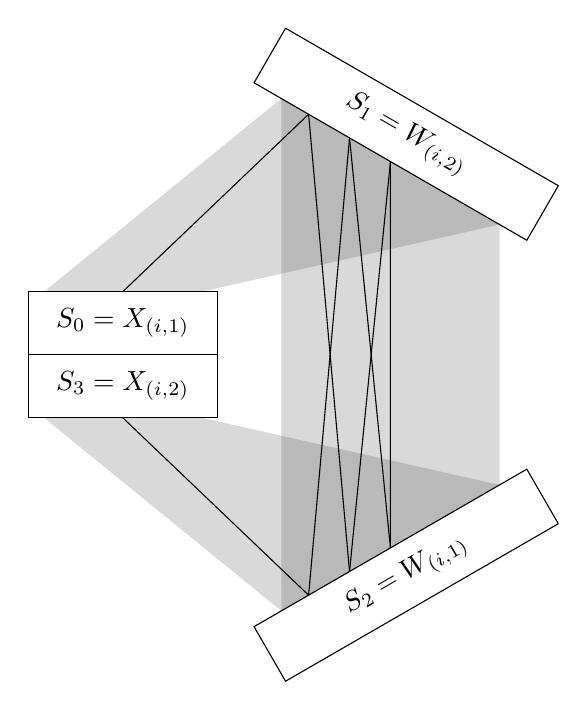
\begin{tikzpicture}[scale=0.8]


\def\sqrt{1.41421356237}

\def\rh{1}
\def\rw{3}

\draw (0,-\rh) -| (\rw,\rh) -| cycle;
\draw (0,0) -- (\rw,0);

\coordinate (xb11) at (\rw-0.25,-\rh);
\coordinate (xb12) at (0.25,-\rh);
\coordinate (xb21) at (0.25,\rh);
\coordinate (xb22) at (\rw-0.25,\rh);
\coordinate (xc1) at (\rw/2,-\rh);
\coordinate (xc2) at (\rw/2,\rh);

\node at (\rw/2,\rh/2) {$S_0=X_{(i,1)}$};
\node at (\rw/2,-\rh/2) {$S_3=X_{(i,2)}$};

\def\rw{5}
\def\rsx{6}
\def\rsy{3.5}
\FPeval{\rshifty2}{\rsy*2}

\def\rx{6}
\def\rr{30}
\FPeval{\rrot2}{\rr+180}

\begin{scope}[shift={(\rsx,-\rsy)},rotate=\rrot2]

\def\rn{1}
\coordinate (r\rn1) at (-\rw/2,0.5){};
\coordinate (r\rn2) at (-\rw/2,-0.5){};
\coordinate (r\rn3) at (\rw/2,-0.5){};
\coordinate (r\rn4) at (\rw/2,0.5){};
\draw (r\rn1) -- (r\rn2) -- (r\rn3) -- (r\rn4) -- (r\rn1);
\coordinate (r{\rn}p1) at (-\rw*0.3,-0.5){};
\coordinate (r{\rn}p2) at (-\rw*0.15,-0.5){};
\coordinate (r{\rn}p3) at (0,-0.5){};
\coordinate (r{\rn}p4) at (\rw*0.15,-0.5){};
\coordinate (r{\rn}p5) at (\rw*0.3,-0.5){};
\coordinate (r{\rn}b1) at (-\rw/2+0.5,-0.5){};
\coordinate (r{\rn}b2) at (\rw/2-0.5,-0.5){};

\fill [opacity=0.15] (xb\rn1) -- (r{\rn}b1) -- (r{\rn}b2) -- (xb\rn2) -- cycle;

\begin{scope}[rotate=-\rrot2]
\begin{scope}[shift={(0,\rshifty2)},rotate=-\rr]

\def\rn{2}
\coordinate (r\rn1) at (-\rw/2,0.5){};
\coordinate (r\rn2) at (-\rw/2,-0.5){};
\coordinate (r\rn3) at (\rw/2,-0.5){};
\coordinate (r\rn4) at (\rw/2,0.5){};
\draw (r\rn1) -- (r\rn2) -- (r\rn3) -- (r\rn4) -- (r\rn1);
\coordinate (r{\rn}p1) at (-\rw*0.3,-0.5){};
\coordinate (r{\rn}p2) at (-\rw*0.15,-0.5){};
\coordinate (r{\rn}p3) at (0,-0.5){};
\coordinate (r{\rn}p4) at (\rw*0.15,-0.5){};
\coordinate (r{\rn}p5) at (\rw*0.3,-0.5){};
\coordinate (r{\rn}b1) at (-\rw/2+0.5,-0.5){};
\coordinate (r{\rn}b2) at (\rw/2-0.5,-0.5){};

\fill [opacity=0.15] (xb\rn1) -- (r{\rn}b1) -- (r{\rn}b2) -- (xb\rn2) -- cycle;

\fill [opacity=0.15] (r{1}b2) -- (r{2}b1) -- (r{2}b2) -- (r{1}b1) -- cycle;
\draw (xc1) -- (r{1}p5);
\draw (r{1}p5)-- (r{2}p2);
\draw (r{2}p2) -- (r{1}p3);
\draw (r{1}p3) -- (r{2}p3);
\draw (r{2}p3) -- (r{1}p4);
\draw (r{1}p4) -- (r{2}p1);
\draw (r{2}p1) -- (xc2);

\end{scope}
\end{scope}

\end{scope}

%}

\node[rotate=\rr] at (\rsx,-\rsy) {$S_2=W_{(i,1)}$};
\node[rotate=-\rr] at (\rsx,\rsy) {$S_1=W_{(i,2)}$};

\end{tikzpicture}
\end{center}

\protect\caption{\label{fig:cluster-paths}An example special path is shown, for $k=7$.}
\end{figure}


Let $n_{i}^{Z}=\left|S_{i}^{Z}\right|=\left|Z_{i}\right|$. Note that
$G_{i}$ is a $\left(\varepsilon_{4},\delta_{4}\right)$-super-regular
blow-up of a 3-cycle $C_{3}$, with part sizes 
\[
n_{i}^{Z},\quad n_{i}^{1}:=\left(\left(k-1\right)/2\right)n_{i}^{Z},\quad n_{i}^{2}:=\left(\left(k-1\right)/2\right)n_{i}^{Z}.
\]
The corresponding complete blow-up $b_{n_{i}^{Z},n_{i}^{1},n_{i}^{2}}\left(C_{3}\right)$
contains $n_{i}^{Z}$ disjoint $k$-cycles (each has a vertex in $S_{i}^{Z}$
and its other $k-1$ vertices alternate between $S_{i}^{1}$ and $S_{i}^{2}$).
By the blow-up lemma, $G_{i}$ also contains $n_{i}^{Z}$ disjoint
$k$-cycles. Since $k$ is odd, each of these must use at least one
vertex from $S_{i}^{Z}$, but since $\left|S_{i}^{Z}\right|=n_{i}^{Z}$,
each cycle must then use exactly one vertex from $S_{i}^{Z}$. These
cycles correspond to special paths which complete our embedding of
$\T$.


\section{Concluding Remarks}

We have proved that any given bounded-degree spanning tree typically
appears when a linear number of random edges are added to a dense
graph. There are a few interesting questions that remain open. Most
prominent is the question of embedding more general kinds of spanning
subgraphs into randomly perturbed graphs. It would be particularly
interesting if the general result of \cite{BST09} (concerning arbitrary
spanning graphs with bounded degree and low bandwidth) could be adapted
to this setting. It is also possible that our use of Szemer\'edi's
regularity lemma could be avoided, thus drastically improving the
constants $\c\left(\a\right)$ and perhaps allowing us to say something
about random perturbations of graphs which have slightly sublinear
minimum degree.

\noindent \textbf{Acknowledgement.} Parts of this work were carried
out when the first author visited the Institute for Mathematical Research
(FIM) of ETH Zurich, and also when the third author visited the School
of Mathematical Sciences of Tel Aviv University, Israel. We would
like to thank both institutions for their hospitality and for creating
a stimulating research environment.

\bibliographystyle{amsplain_initials}
\bibliography{references}

\end{document}
